\documentclass[11pt]{article}
\usepackage[preprint]{acl}
\usepackage{times}
\usepackage[T1]{fontenc}
\usepackage{graphicx}
\usepackage{microtype}
\usepackage{inconsolata}
\title{Figure placement test}
\author{Test}
\begin{document}
\maketitle
\section{Introduction}
Agents that hold a shell can write the record of their own actions. We remove
that record from the trust path: a kernel probe attributes each file touch to an
agent by cgroup inode, and two agents touching the same object become an edge.
The sentence here exists only to establish body text at the same size as the
caption, so the comparison against the figure labels is honest. Body text in this
template is set at eleven points on a measure of six and a half inches, which is
what a reader will see beside the figure in the finished paper.

\begin{figure*}[t]
\centering
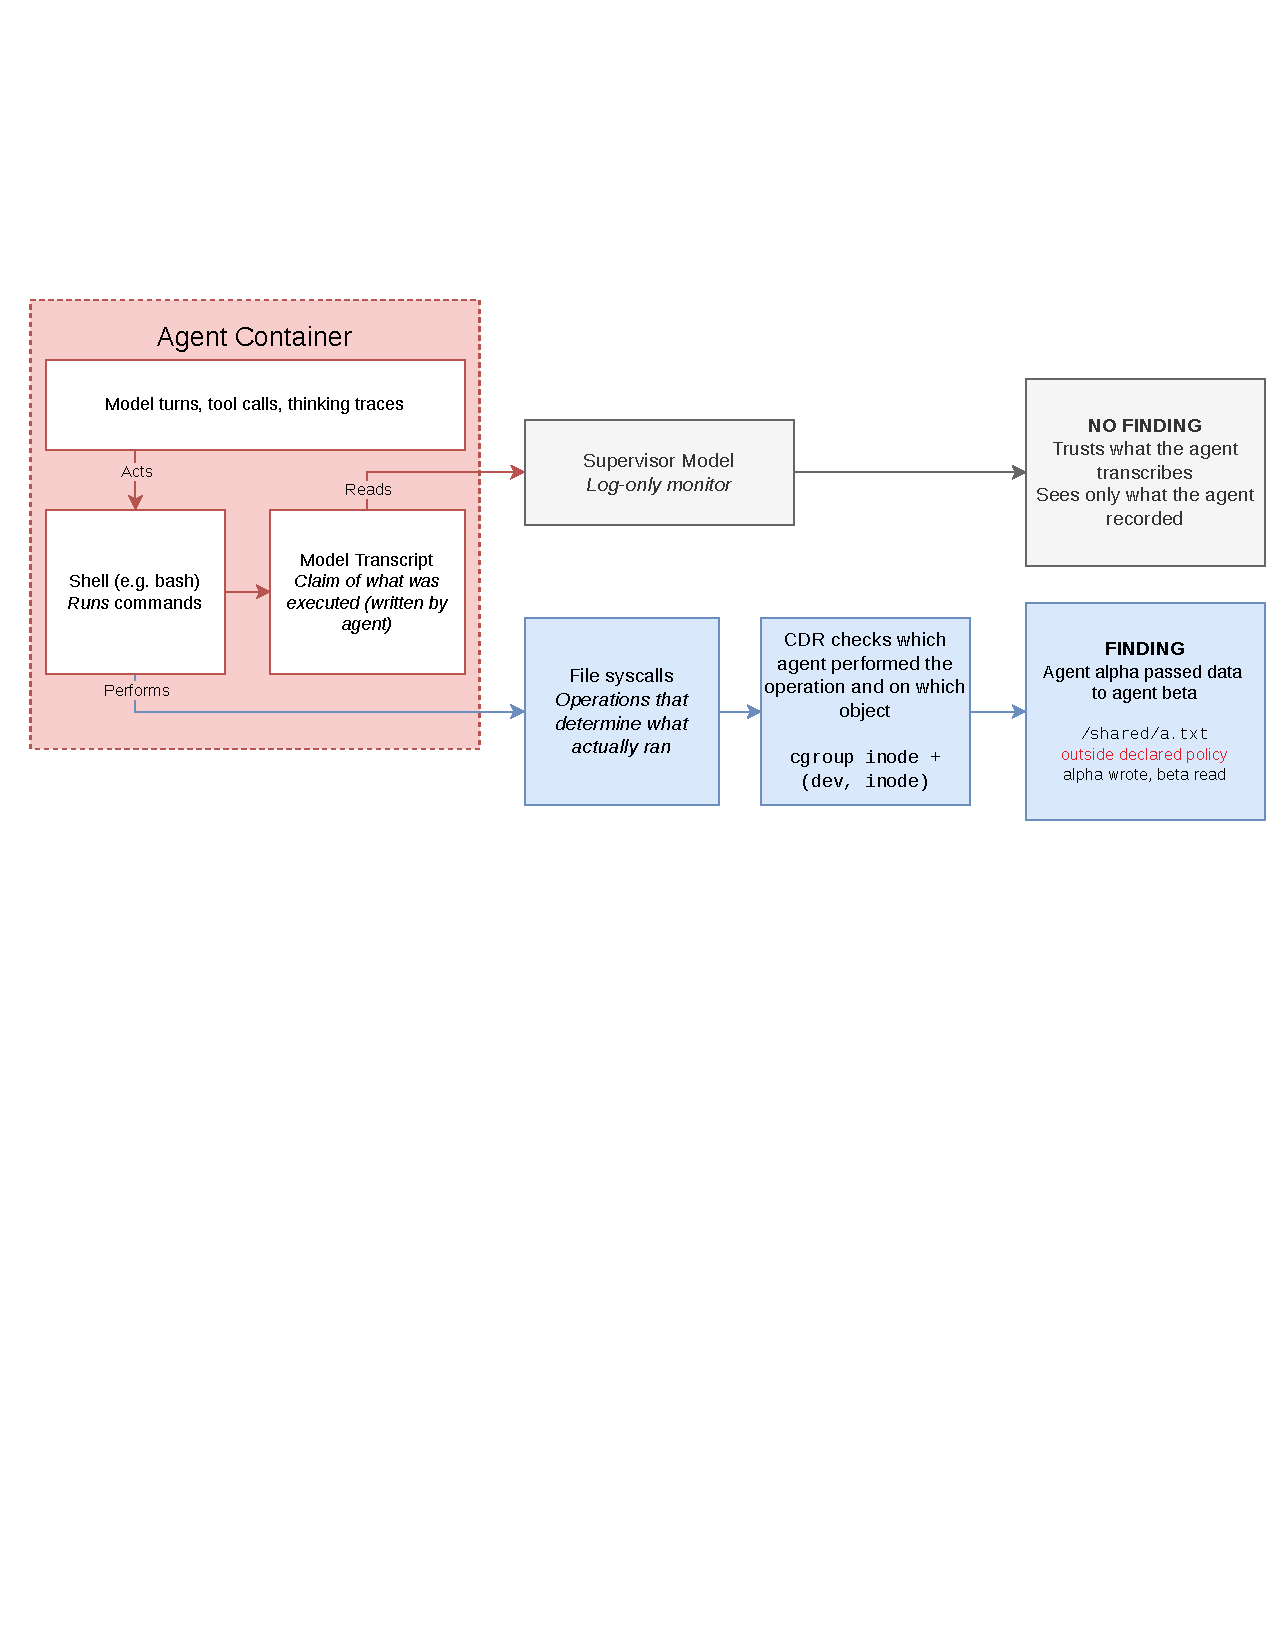
\includegraphics[width=\textwidth]{figures/fig1.pdf}
\caption{One action produces two records. Left of the dashed line everything is
written by the agent and can be rewritten by it; the log-only monitor has no
other input, so it sees the claim and reports nothing. Right of the line the
kernel witnesses the syscall, resolves who acted and on what, and the correlator
emits an edge. The object is identified by device and inode rather than by path.}
\label{fig:trust}
\end{figure*}

\noindent Body text after the figure. The caption is the standard test: if the
figure labels are legible at the same reading distance as this paragraph when the
PDF is viewed at one hundred percent, the figure will survive print and screen.

\section{More text so the float lands naturally}
This paragraph exists so the page has enough body copy to receive a top float in
the way the finished paper will. A full-width figure consumes a band across both
columns, and the thing worth checking is whether the band sits comfortably
against the surrounding measure, whether the caption is readable at the same
distance as the body, and whether the figure's internal type survives contact
with the page rather than only looking right on its own.

The second consideration is vertical cost. On an eight page budget, a full-width
figure that occupies a quarter of a page is expensive, and it has to earn that
space by replacing prose rather than duplicating it. This figure replaces the
paragraph that would otherwise have to explain the trust boundary, the monitor's
input, and the object key, so the trade is favourable.

The third is legibility at reproduction. Reviewers read PDFs on laptops and
occasionally print them. Type below six points fails the second case and often
the first, which is why the labels here are set no smaller than 5.8 points and
the two most important ones, the monitor's conclusion and the verdict, are set
larger and heavier than their neighbours.


\section{Placement check two}
Full-width floats are judged against the measure they displace, so this section
adds enough body copy for the page to be read as a page rather than as a frame
around a figure. The question a reader will actually ask is whether the diagram
earns its band: if the caption is doing the work the picture cannot, the picture
should shrink or go. Here the picture carries the claim, the caption carries the
consequence, and the body carries the mechanism, which is the right division.

A second reason to look at a populated page is float interaction. Two-column
documents place a spanning float at the top of a page and resume text beneath it,
and the resume is where the reading rhythm either holds or breaks. If the band is
too tall the columns restart far down the page and the reader loses the thread
between the paragraph before and the paragraph after.

The third reason is that captions in this template run at nine point, so the
figure's internal type must sit at or below that without collapsing. Anything at
five points or smaller reads as texture at a hundred percent zoom, which is the
only zoom that matters for a reviewer skimming a PDF on a laptop.



\end{document}
